\documentclass[tikz,border=8pt]{standalone}
\usepackage{tikz}
\usepackage{pgfplots}
\usepackage{amsmath,amssymb}
\usepackage[T1]{fontenc}
\usepackage{lmodern}
\usepackage{xcolor}
\usetikzlibrary{arrows.meta,positioning,shapes.geometric,fit,calc,backgrounds,matrix}
\pgfplotsset{compat=1.18}
\definecolor{ink}{HTML}{18202A}
\definecolor{blue}{HTML}{2563EB}
\definecolor{bluefill}{HTML}{EAF1FF}
\definecolor{green}{HTML}{14804A}
\definecolor{greenfill}{HTML}{E8F6EE}
\definecolor{amber}{HTML}{B56A00}
\definecolor{amberfill}{HTML}{FFF3D6}
\definecolor{red}{HTML}{B42318}
\definecolor{redfill}{HTML}{FDECEC}
\definecolor{gray}{HTML}{667085}
\definecolor{light}{HTML}{F4F6F8}
\definecolor{linegray}{HTML}{C7CDD4}
\tikzset{
  box/.style={draw=ink, rounded corners=3pt, very thick, fill=white, align=center, inner sep=7pt, font=\sffamily\small},
  bluebox/.style={box, fill=bluefill, draw=blue},
  greenbox/.style={box, fill=greenfill, draw=green},
  amberbox/.style={box, fill=amberfill, draw=amber},
  redbox/.style={box, fill=redfill, draw=red},
  ghost/.style={draw=linegray, rounded corners=3pt, thick, fill=light, align=center, inner sep=7pt, font=\sffamily\small},
  label/.style={font=\sffamily\footnotesize, text=gray, align=center},
  title/.style={font=\sffamily\bfseries\large, text=ink, align=center},
  arrow/.style={-{Latex[length=3mm,width=2mm]}, very thick, draw=ink},
  bluearrow/.style={-{Latex[length=3mm,width=2mm]}, very thick, draw=blue},
  redarrow/.style={-{Latex[length=3mm,width=2mm]}, very thick, draw=red},
  greenarrow/.style={-{Latex[length=3mm,width=2mm]}, very thick, draw=green}
}

\begin{document}
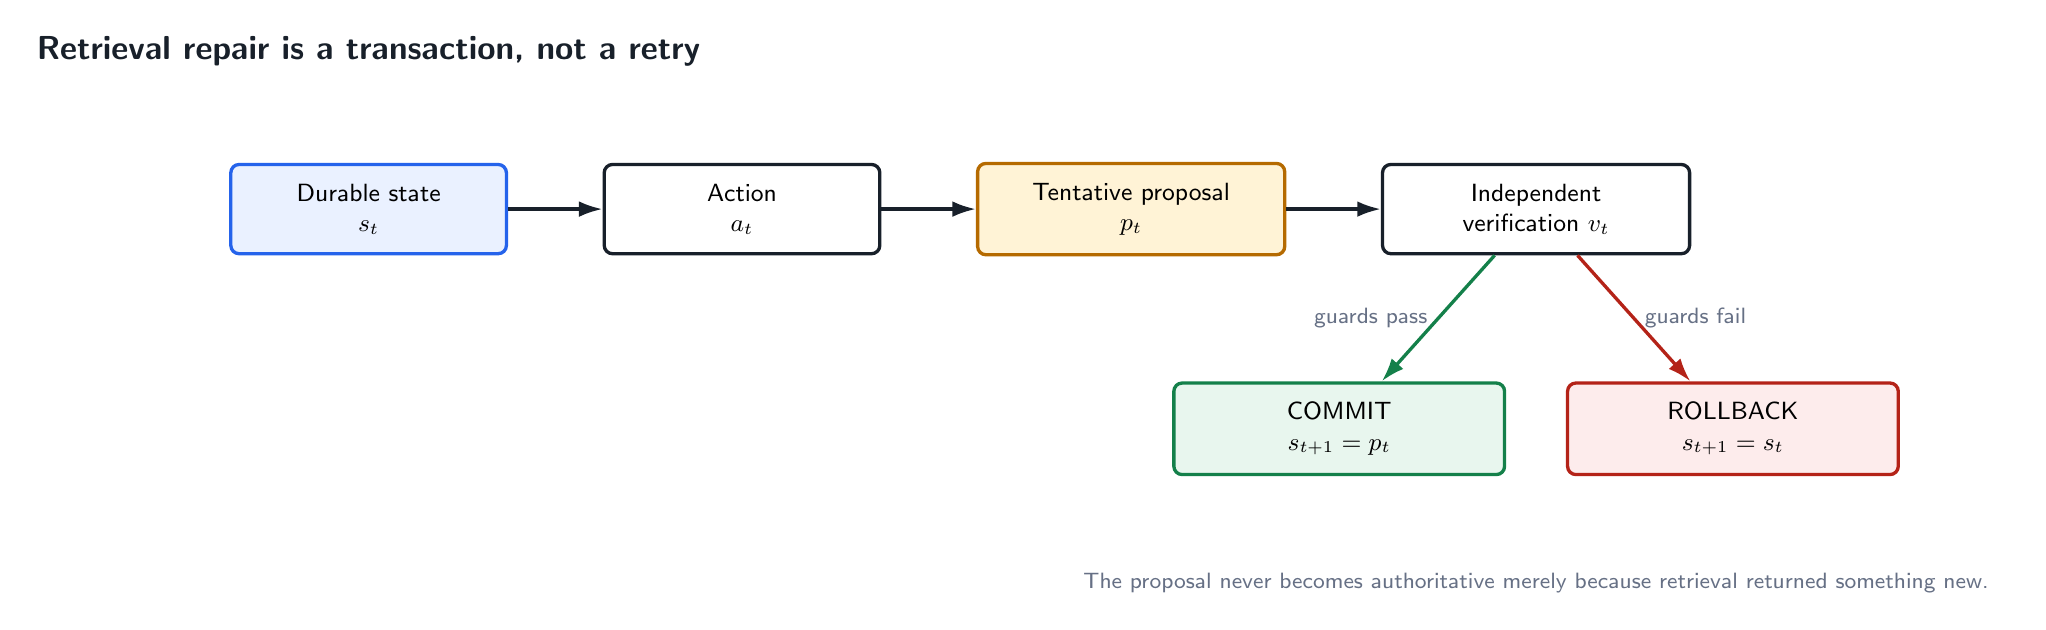
\begin{tikzpicture}[node distance=10mm and 12mm]
\node[title] (ttl) {Retrieval repair is a transaction, not a retry};
\node[bluebox, below=11mm of ttl, minimum width=35mm] (s) {Durable state\\$s_t$};
\node[box, right=of s, minimum width=35mm] (a) {Action\\$a_t$};
\node[amberbox, right=of a, minimum width=39mm] (p) {Tentative proposal\\$p_t$};
\node[box, right=of p, minimum width=39mm] (v) {Independent\\verification $v_t$};
\draw[arrow] (s)--(a); \draw[arrow] (a)--(p); \draw[arrow] (p)--(v);
\node[greenbox, below=16mm of v, xshift=-25mm, minimum width=42mm] (c) {COMMIT\\$s_{t+1}=p_t$};
\node[redbox, below=16mm of v, xshift=25mm, minimum width=42mm] (rb) {ROLLBACK\\$s_{t+1}=s_t$};
\draw[greenarrow] (v)--node[label,left]{guards pass}(c);
\draw[redarrow] (v)--node[label,right]{guards fail}(rb);
\node[label, below=11mm of c, xshift=25mm, text width=120mm] {The proposal never becomes authoritative merely because retrieval returned something new.};
\end{tikzpicture}
\end{document}
